\chapter{Results}\label{Results}
\section{1D Bose Polaron in the Heavy Impurity Limit}
\begin{figure}[H]
    \centering
    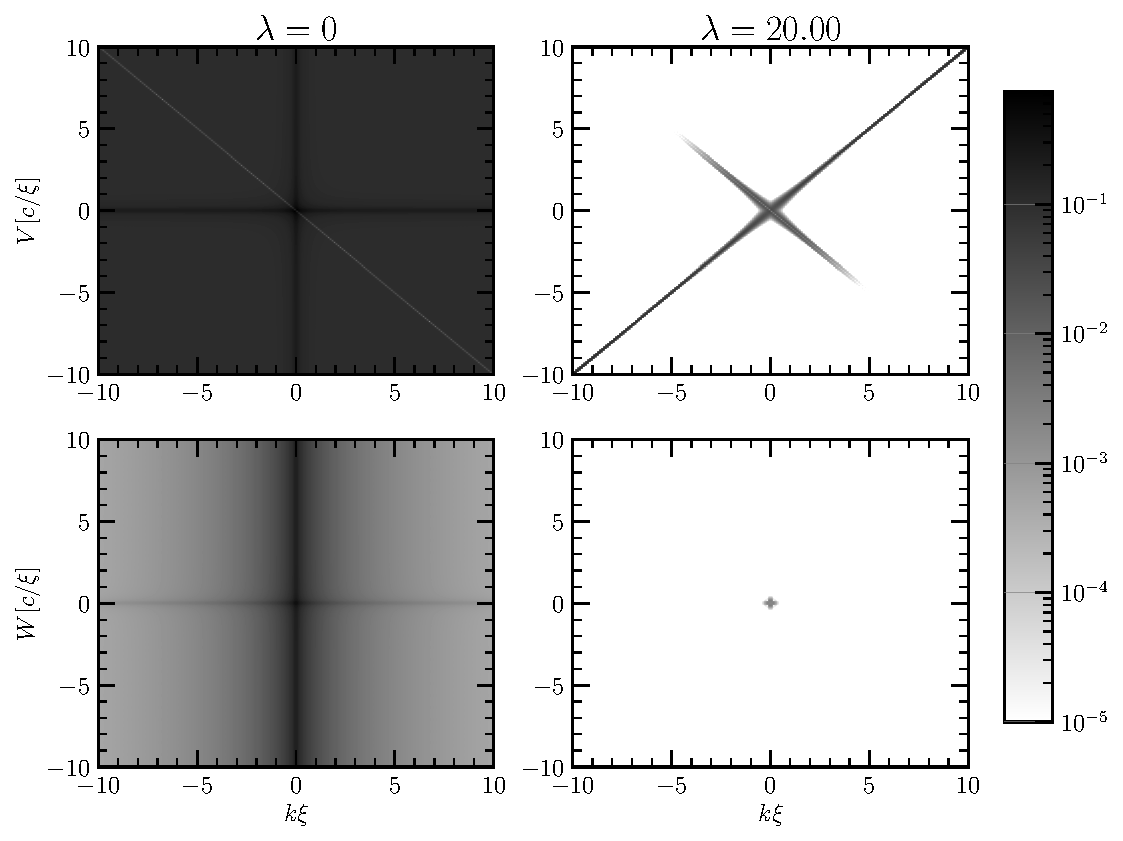
\includegraphics{figures/plots/PDF/FlowIllustration.pdf}
    \caption{Visualization of how the flow progresses for $\eta=10$ by shading larger absolute values for $V_{k,k^\prime},W_{k,k^\prime}$ darker. We see that good suppression occurs for all $W_{k,k^\prime}$, with slower convergence for smaller $|k|,|k^\prime|$.  The matrix elements near the diagonal $V_{k,k}$ decay significantly slower than most off-diagonal elements. All matrix elements $V_{k,-k}$ converge, but to a value different from zero.}
    \label{FlowIllustration}
\end{figure}
As seen in figure \ref{FlowIllustration}